\documentclass[a4paper,oneside,12pt]{report}
% Package yang diperlukan
\usepackage{graphicx}      % Untuk memasukkan gambar
\usepackage{geometry}      % Untuk mengatur margin halaman
\usepackage{listings}      % Untuk menampilkan blok kode
\usepackage{xcolor}        % Untuk menggunakan warna
\usepackage{float}         % Untuk kontrol penempatan float (seperti gambar)
\usepackage{hyperref}      % Untuk membuat hyperlink (URL, referensi)
\usepackage{natbib}        % Untuk citation dengan \cite{} yang clickable
\usepackage{indentfirst}   % Untuk memberi indentasi pada paragraf pertama setiap seksi
\usepackage{url}           % Untuk format URL
\usepackage{fancyhdr}      % Untuk kustomisasi header dan footer
\usepackage{tocloft}       % Untuk kustomisasi Daftar Isi
\usepackage{bookmark}      % Untuk manajemen bookmark PDF yang lebih baik

%======================================================================
% PENGATURAN GEOMETRI HALAMAN
%======================================================================
% Margin umum untuk isi laporan
\geometry{left=3cm, right=2.5cm, top=2cm, bottom=2.5cm}
\sloppy

%======================================================================
% PENGATURAN WARNA UNTUK BLOK KODE
%======================================================================
\definecolor{codegreen}{rgb}{0,0.6,0}
\definecolor{codegray}{rgb}{0.5,0.5,0.5}
\definecolor{codepurple}{rgb}{0.58,0,0.82}
\definecolor{backcolour}{rgb}{0.95,0.95,0.92}
\definecolor{darkblue}{rgb}{0,0,0.6}

%======================================================================
% PENGATURAN BLOK KODE (LISTINGS)
%======================================================================
% Gaya umum untuk semua blok kode
\lstdefinestyle{commonstyle}{
    backgroundcolor=\color{backcolour}, 
    breakatwhitespace=false, 
    breaklines=true, 
    captionpos=b, 
    keepspaces=true,
    numbers=left, 
    numbersep=5pt, 
    showspaces=false, 
    showstringspaces=false,
    showtabs=false, 
    tabsize=2, 
    frame=single,
    basicstyle=\ttfamily\footnotesize,
    numberstyle=\tiny\color{codegray},
    columns=flexible,
    postbreak=\mbox{\textcolor{red}{$\hookrightarrow$}\space},
    breakindent=0pt,
    breakautoindent=false
}

% Gaya khusus untuk HTML
\lstdefinestyle{htmlstyle}{
    style=commonstyle,
    language=HTML,
    commentstyle=\color{codegreen},
    keywordstyle=\color{codepurple},
    stringstyle=\color{codegreen},
    basicstyle=\ttfamily\scriptsize
}

% Gaya khusus untuk CSS
\lstdefinestyle{cssstyle}{
    style=commonstyle,
    commentstyle=\color{codegreen},
    keywordstyle=\color{darkblue},
    stringstyle=\color{codepurple},
    emph={color, background, font, margin, padding, border, display, position, width, height},
    emphstyle=\color{darkblue},
    basicstyle=\ttfamily\scriptsize
}

% Gaya khusus untuk Python
\lstdefinestyle{pythonstyle}{
    style=commonstyle,
    language=Python,
    commentstyle=\color{codegreen},
    keywordstyle=\color{darkblue},
    stringstyle=\color{codepurple},
    emph={import,from,class,def,for,while,if,else,elif,try,except,finally},
    emphstyle=\color{darkblue}
}

% Gaya khusus untuk SQL
\lstdefinestyle{sqlstyle}{
    style=commonstyle,
    language=SQL,
    commentstyle=\color{codegreen},
    keywordstyle=\color{darkblue},
    stringstyle=\color{codepurple},
    emph={SELECT,FROM,WHERE,INSERT,UPDATE,DELETE,CREATE,DROP},
    emphstyle=\color{darkblue}
}

% Gaya khusus untuk JavaScript
\lstdefinestyle{javascriptstyle}{
    style=commonstyle,
    language=JavaScript,
    commentstyle=\color{codegreen},
    keywordstyle=\color{darkblue},
    stringstyle=\color{codepurple},
    emph={function,var,let,const,return,if,for,while,do,else,switch,case},
    emphstyle=\color{darkblue}
}

% Gaya khusus untuk Java
\lstdefinestyle{javastyle}{
    style=commonstyle,
    language=Java,
    commentstyle=\color{codegreen},
    keywordstyle=\color{darkblue}\bfseries,
    stringstyle=\color{codepurple},
    emph={@Test,@Mock,@InjectMocks,@ExtendWith},
    emphstyle=\color{codepurple}
}

%======================================================================
% PENGATURAN LAIN-LAIN
%======================================================================

% Mengganti nama default "Figure" menjadi "Gambar"
\renewcommand{\figurename}{Gambar}
\renewcommand{\thefigure}{\arabic{figure}}

% Pengaturan Hyperlink
\hypersetup{
    colorlinks=true, 
    linkcolor=black, 
    filecolor=black, 
    urlcolor=black,
    citecolor=blue,
    pdftitle={Laporan Praktikum}, 
    pdfpagemode=FullScreen, 
    breaklinks=true
}

% Pengaturan citation style
\bibliographystyle{plain}

% Pengaturan Header & Footer (nomor halaman di tengah bawah)
\pagestyle{fancy}
\fancyhf{}
\fancyfoot[C]{\thepage}
\renewcommand{\headrulewidth}{0pt}

\fancypagestyle{plain}{
    \fancyhf{}
    \fancyfoot[C]{\thepage}
    \renewcommand{\headrulewidth}{0pt}
}

%======================================================================
% PENGATURAN STRUKTUR BAB DAN DAFTAR ISI
%======================================================================
\renewcommand{\contentsname}{Daftar Isi}
\renewcommand{\bibname}{Daftar Pustaka}

% Menghilangkan nomor bab tetapi mempertahankan penomoran seksi
\renewcommand{\thechapter}{}
\renewcommand{\chaptername}{}

% Format penomoran seksi menjadi [nomor bab].[nomor seksi]
\renewcommand{\thesection}{\arabic{chapter}.\arabic{section}}
\renewcommand{\thesubsection}{\thesection.\arabic{subsection}}

\setcounter{secnumdepth}{3}
\setcounter{tocdepth}{2}

% Format Daftar Isi (TOC)
\renewcommand{\cftchapdotsep}{\cftdotsep}
\renewcommand{\cftchapleader}{\cftdotfill{\cftchapdotsep}}
\setlength{\cftchapindent}{0em}
\setlength{\cftsecindent}{2em}
\setlength{\cftsubsecindent}{4em}
\setlength{\cftchapnumwidth}{0em}
\setlength{\cftsecnumwidth}{2.5em}
\setlength{\cftsubsecnumwidth}{3.2em}
\renewcommand{\cftchappresnum}{}
\renewcommand{\cftchapaftersnum}{}

% Perintah kustom untuk membuat judul bab di TOC menjadi tebal
\newcommand{\tocboldsection}[1]{%
  \protect\renewcommand{\protect\cftchapfont}{\protect\bfseries}%
  #1%
  \protect\renewcommand{\protect\cftchapfont}{}%
}

%======================================================================
% AWAL DOKUMEN
%======================================================================
\begin{document}

% Halaman Judul
\newgeometry{left=3cm, right=2.5cm, top=2.5cm, bottom=3cm}
\begin{titlepage}
\begin{center}
\vspace*{0.5cm}
{\large \textbf{\MakeUppercase{Laporan Praktikum}}} \\[0.4cm]
{\large \textbf{\MakeUppercase{PRAKTIKUM PENGUJIAN PERANGKAT LUNAK}}} \\[0.4cm]
{\large \textbf{\MakeUppercase{Pertemuan 4}}} \\[0.4cm]
{\large \textbf{\MakeUppercase{MOCK, SPY, DAN STUB TESTING MENGGUNAKAN MOCKITO}}} \\[1.5cm]


\includegraphics[height=7cm]{lambang ugm.png} \\[1cm]

{\normalsize \textbf{Disusun oleh:}} \\[0.4cm]
\begin{tabular}{@{}l l @{}}
  \textbf{Nama}           & : Januarsyah Akbar \\
  \textbf{NIM}            & : 24/535846/SV/24314 \\
  \textbf{Kelas}          & : PL4B2 \\
    \textbf{Dosen Pengampu} & : Divi Galih Prasetyo Putri, S.Kom., M.Kom., Ph.D.
\end{tabular} \\[1.2cm]

{\normalsize \textbf{PROGRAM STUDI D-IV}} \\[0.2cm]
{\normalsize \textbf{TEKNOLOGI REKAYASA PERANGKAT LUNAK}} \\[0.2cm]
{\normalsize \textbf{DEPARTEMEN TEKNIK ELEKTRO DAN INFORMATIKA}} \\[0.2cm]
{\normalsize \textbf{SEKOLAH VOKASI}} \\[0.2cm]
{\normalsize \textbf{UNIVERSITAS GADJAH MADA}} \\[0.2cm]
{\normalsize \textbf{YOGYAKARTA}} \\[0.2cm]
{\normalsize \textbf{\today}} \\[1.2cm]
\end{center}
\end{titlepage}
\restoregeometry

\thispagestyle{empty}
\clearpage
\stepcounter{page}
\thispagestyle{empty}

% --- Daftar Isi ---
\addcontentsline{toc}{chapter}{Daftar Isi}
\tableofcontents
\clearpage

% Mengatur penomoran halaman menjadi arab dan mulai dari 3
\pagenumbering{arabic}
\setcounter{page}{3}

%======================================================================
\chapter[Tujuan Praktikum]{Tujuan Praktikum}
%======================================================================
\begin{enumerate}
   \item Mahasiswa mampu memahami konsep dan perbedaan antara Mock, Spy, dan Stub dalam pengujian perangkat lunak.
   \item Mahasiswa mampu mengimplementasikan Mock, Spy, dan Stub menggunakan framework Mockito pada proyek Java.
   \item Mahasiswa mampu melakukan verifikasi interaksi dan verifikasi state dalam unit test menggunakan anotasi dan metode Mockito.
\end{enumerate}
\clearpage

%======================================================================
\chapter[\tocboldsection{Hasil dan Pembahasan}]{Hasil dan Pembahasan}
%======================================================================

%----------------------------------------------------------------------
\section{Langkah Praktikum}
%----------------------------------------------------------------------

Pada langkah praktikum ini, dilakukan implementasi tiga teknik pengujian berbasis Mockito, yaitu \textbf{Mock}, \textbf{Spy}, dan \textbf{Stub}. Sebelum menjalankan pengujian, disiapkan terlebih dahulu kelas pendukung \texttt{User}, \texttt{UserRepository}, dan \texttt{UserService}.

% ---- Supporting classes ----
\subsection{Kelas Pendukung}

Kelas \texttt{User} merupakan model data pengguna dengan atribut \texttt{id} dan \texttt{name}.

\begin{lstlisting}[style=javastyle, caption={User.java}]
public class User {
    public String id;
    public String name;

    public User(String id, String name) {
        this.id = id;
        this.name = name;
    }
}
\end{lstlisting}

\texttt{UserRepository} adalah antarmuka (interface) yang menyediakan operasi \texttt{save} dan \texttt{findById}.

\begin{lstlisting}[style=javastyle, caption={UserRepository.java}]
public interface UserRepository {
    void save(User user);
    User findById(String id);
}
\end{lstlisting}

\texttt{UserService} berisi logika bisnis, yaitu mendaftarkan pengguna dan mengambil nama pengguna berdasarkan ID.

\begin{lstlisting}[style=javastyle, caption={UserService.java}]
public class UserService {
    private final UserRepository repository;

    public UserService(UserRepository repository) {
        this.repository = repository;
    }

    public void register(User user) {
        repository.save(user);
    }

    public String getUserName(String id) {
        User user = repository.findById(id);
        return user.name;
    }
}
\end{lstlisting}

% ---- Mock Test ----
\subsection{Mock Test}

\textbf{Mock} adalah objek tiruan yang sepenuhnya dikendalikan oleh framework Mockito. Seluruh metodenya mengembalikan nilai default dan tidak menjalankan implementasi nyata. Mock digunakan untuk \textit{verifikasi interaksi}, yaitu memastikan bahwa metode tertentu dipanggil (atau tidak dipanggil) selama eksekusi.

\begin{lstlisting}[style=javastyle, caption={MockTest.java}]
import org.junit.jupiter.api.Test;
import static org.mockito.Mockito.*;

public class MockTest {
    @Test
    public void testMock(){
        UserRepository mockRepo = mock(UserRepository.class);
        UserService userService = new UserService(mockRepo);
        User user = new User("A01","Budiono");

        userService.register(user);

        verify(mockRepo, times(1)).save(user);

        verify(mockRepo, never()).findById(anyString());
    }
}
\end{lstlisting}

Pada pengujian di atas, objek \texttt{mockRepo} dibuat sebagai mock dari \texttt{UserRepository}. Setelah metode \texttt{register(user)} dipanggil, dilakukan dua verifikasi interaksi:
\begin{enumerate}
    \item \texttt{verify(mockRepo, times(1)).save(user)} --- memastikan bahwa metode \texttt{save} dipanggil tepat satu kali dengan argumen \texttt{user}.
    \item \texttt{verify(mockRepo, never()).findById(anyString())} --- memastikan bahwa metode \texttt{findById} \textit{tidak pernah} dipanggil selama proses registrasi.
\end{enumerate}

\begin{figure}[H]
    \centering
    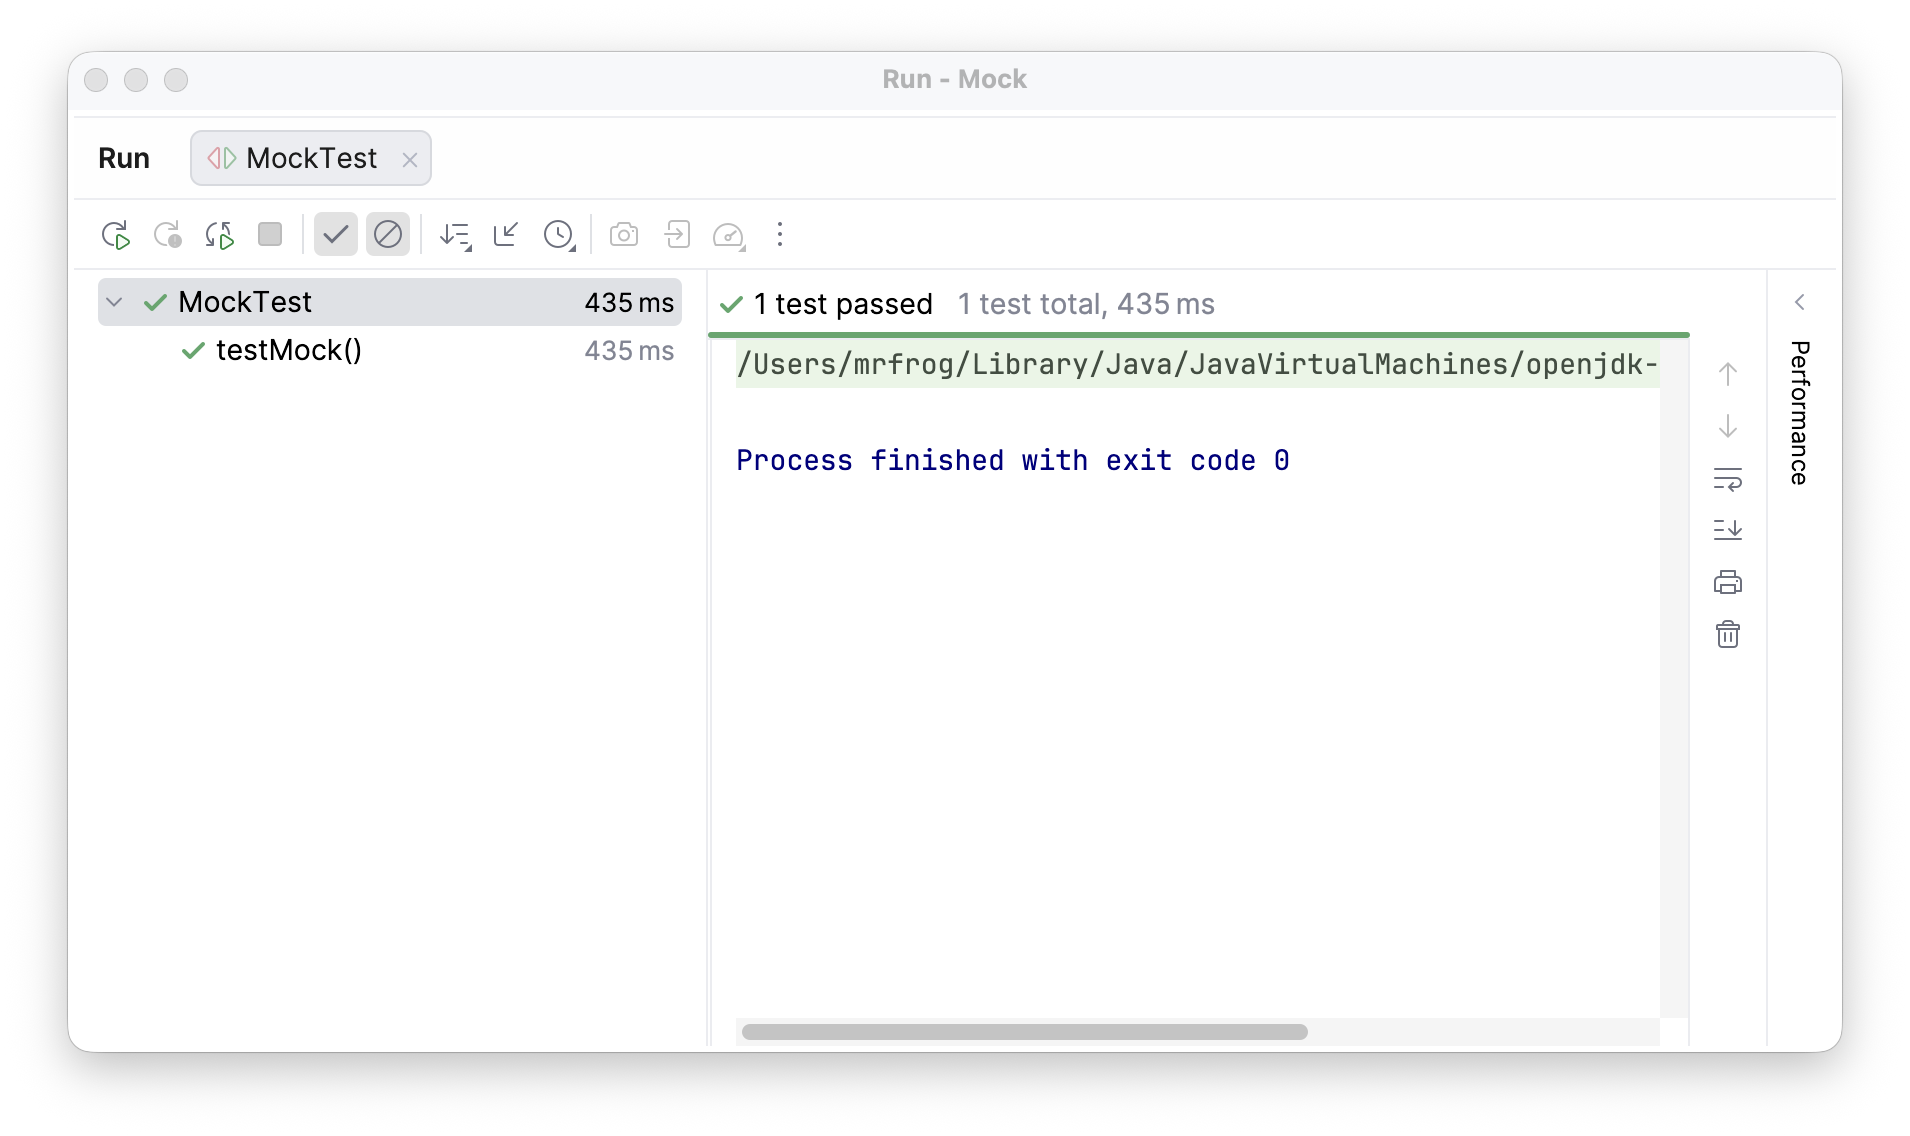
\includegraphics[width=0.9\textwidth]{mocktest.png}
    \caption{Hasil eksekusi MockTest}
\end{figure}

% ---- Spy Test ----
\subsection{Spy Test}

\textbf{Spy} adalah pembungkus (\textit{wrapper}) dari objek nyata. Berbeda dengan Mock, Spy menjalankan implementasi asli dari objek yang dibungkusnya, kecuali pada metode yang secara eksplisit di-\textit{stub}. Spy cocok digunakan ketika ingin melakukan verifikasi interaksi sekaligus mempertahankan perilaku nyata dari objek.

\begin{lstlisting}[style=javastyle, caption={SpyTest.java}]
import org.junit.jupiter.api.Test;
import java.util.ArrayList;
import java.util.List;
import static org.junit.jupiter.api.Assertions.assertEquals;
import static org.mockito.Mockito.spy;
import static org.mockito.Mockito.verify;

public class SpyTest {
    @Test
    public void spyTest(){
        // 1. setup spy
        List<String> realList = new ArrayList<>();
        List<String> spyList  = spy(realList);

        // 2. execution
        spyList.add("A01");
        spyList.add("A02");

        // 3. state verification
        assertEquals(2, spyList.size());
        assertEquals("A01", spyList.get(0));

        // 4. interaction verification
        verify(spyList).add("A02");
        verify(spyList).add("A01");
    }
}
\end{lstlisting}

Langkah-langkah pengujian Spy:
\begin{enumerate}
    \item \textbf{Setup Spy} --- dibuat objek \texttt{ArrayList} nyata, kemudian dibungkus dengan \texttt{spy()}.
    \item \textbf{Eksekusi} --- dua elemen ditambahkan ke \texttt{spyList}. Karena ini Spy, metode \texttt{add} yang asli benar-benar dieksekusi.
    \item \textbf{Verifikasi State} --- memastikan ukuran list adalah 2 dan elemen pertama adalah \texttt{"A01"}.
    \item \textbf{Verifikasi Interaksi} --- memastikan \texttt{add("A01")} dan \texttt{add("A02")} memang pernah dipanggil.
\end{enumerate}

\begin{figure}[H]
    \centering
    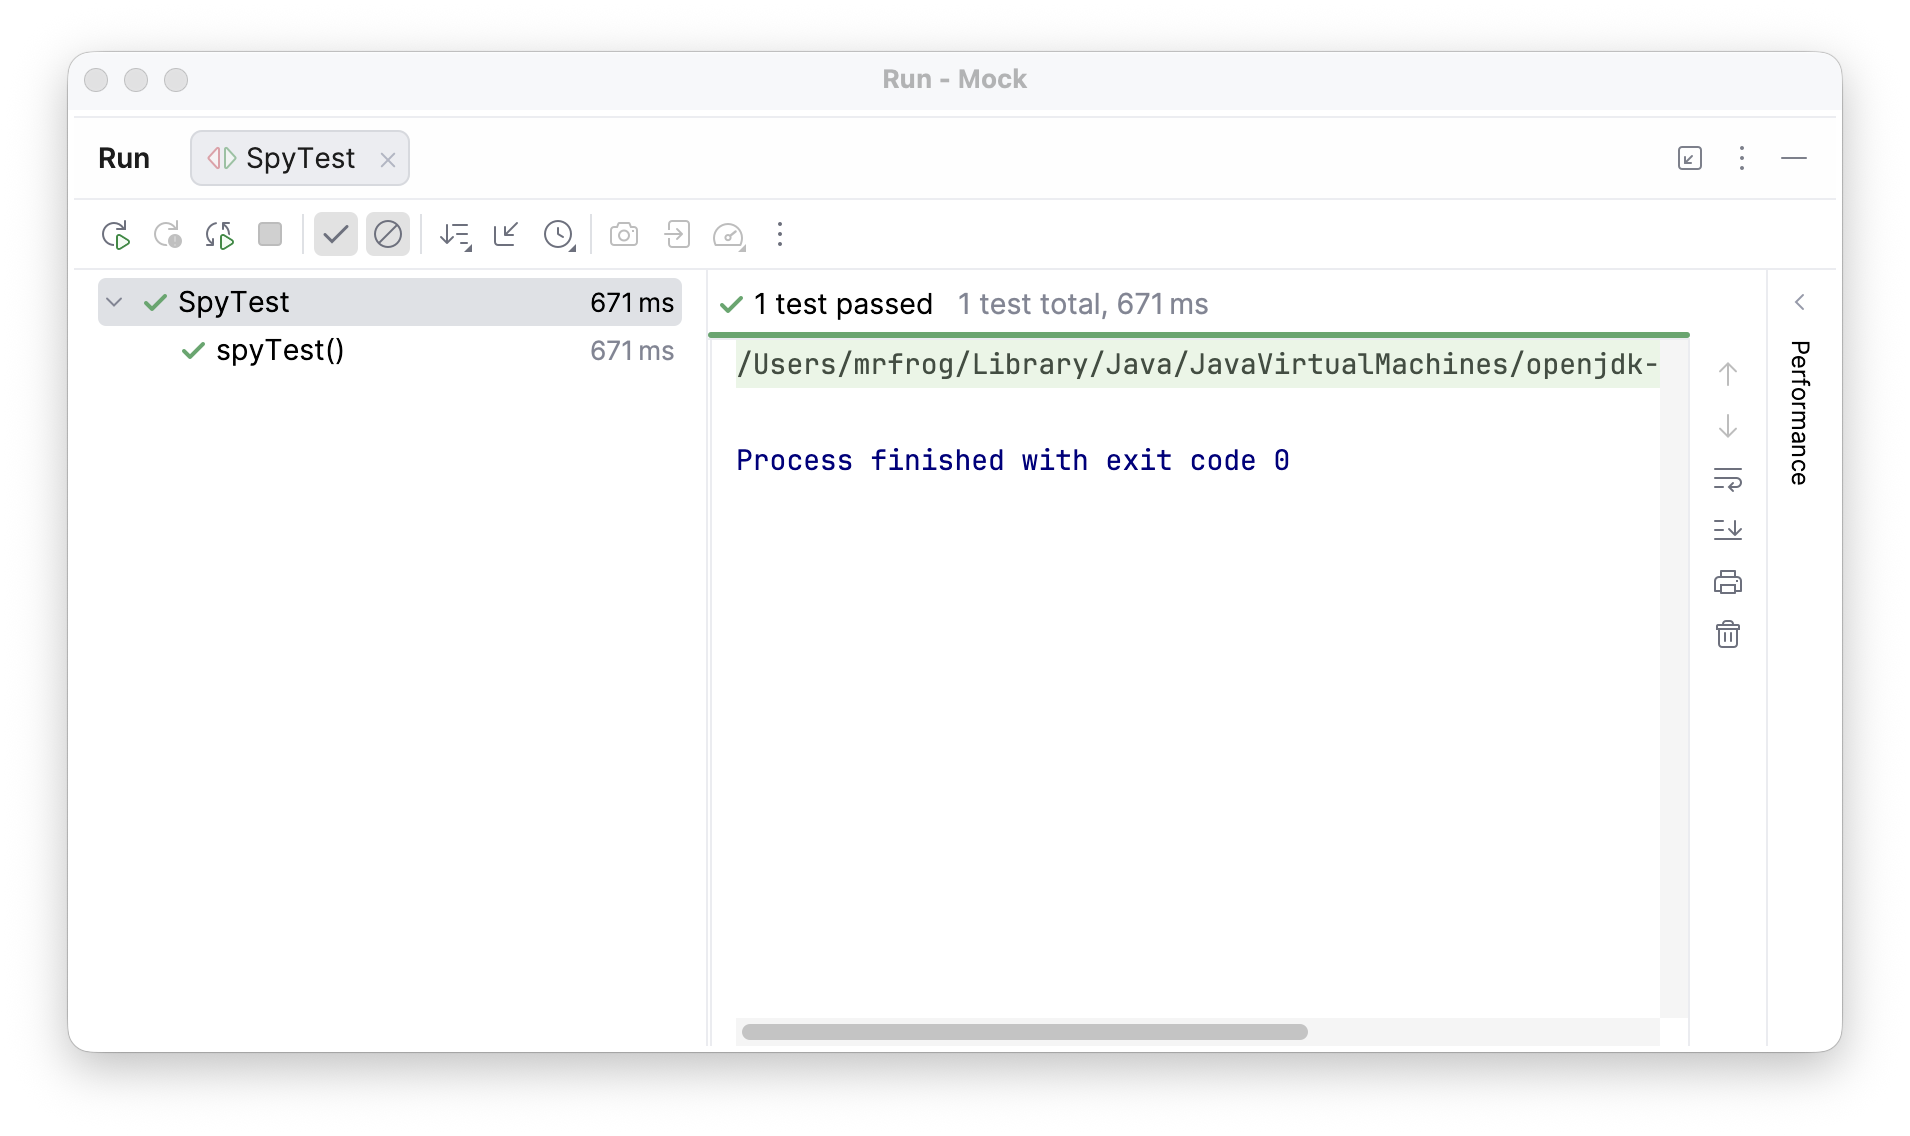
\includegraphics[width=0.9\textwidth]{spytest.png}
    \caption{Hasil eksekusi SpyTest}
\end{figure}

% ---- Stub Test ----
\subsection{Stub Test}

\textbf{Stub} adalah objek tiruan yang dikonfigurasi untuk mengembalikan nilai tertentu saat metode tertentu dipanggil. Stub digunakan untuk \textit{verifikasi state}, yaitu memeriksa kebenaran nilai yang dihasilkan oleh unit yang sedang diuji, tanpa memperhatikan bagaimana objek dependensinya dipanggil.

\begin{lstlisting}[style=javastyle, caption={StubTest.java}]
import org.junit.jupiter.api.Test;
import static org.junit.jupiter.api.Assertions.assertEquals;
import static org.mockito.Mockito.mock;
import static org.mockito.Mockito.when;

public class StubTest {
    @Test
    public void test() {
        // 1. setup stub (tiruan)
        UserRepository stubRepo = mock(UserRepository.class);

        // 2. setup stubing
        User fakeUser = new User("A01", "Budiono");
        when(stubRepo.findById("A01")).thenReturn(fakeUser);

        // 3. service test
        UserService service = new UserService(stubRepo);
        String name = service.getUserName("A01");

        assertEquals(name, fakeUser.name);
    }
}
\end{lstlisting}

Pada pengujian Stub:
\begin{enumerate}
    \item \texttt{stubRepo} dibuat sebagai mock dari \texttt{UserRepository}.
    \item Dikonfigurasi agar \texttt{findById("A01")} mengembalikan objek \texttt{fakeUser}.
    \item \texttt{UserService.getUserName("A01")} dipanggil, dan hasilnya diverifikasi sama dengan \texttt{fakeUser.name}, yaitu \texttt{"Budiono"}.
\end{enumerate}

\begin{figure}[H]
    \centering
    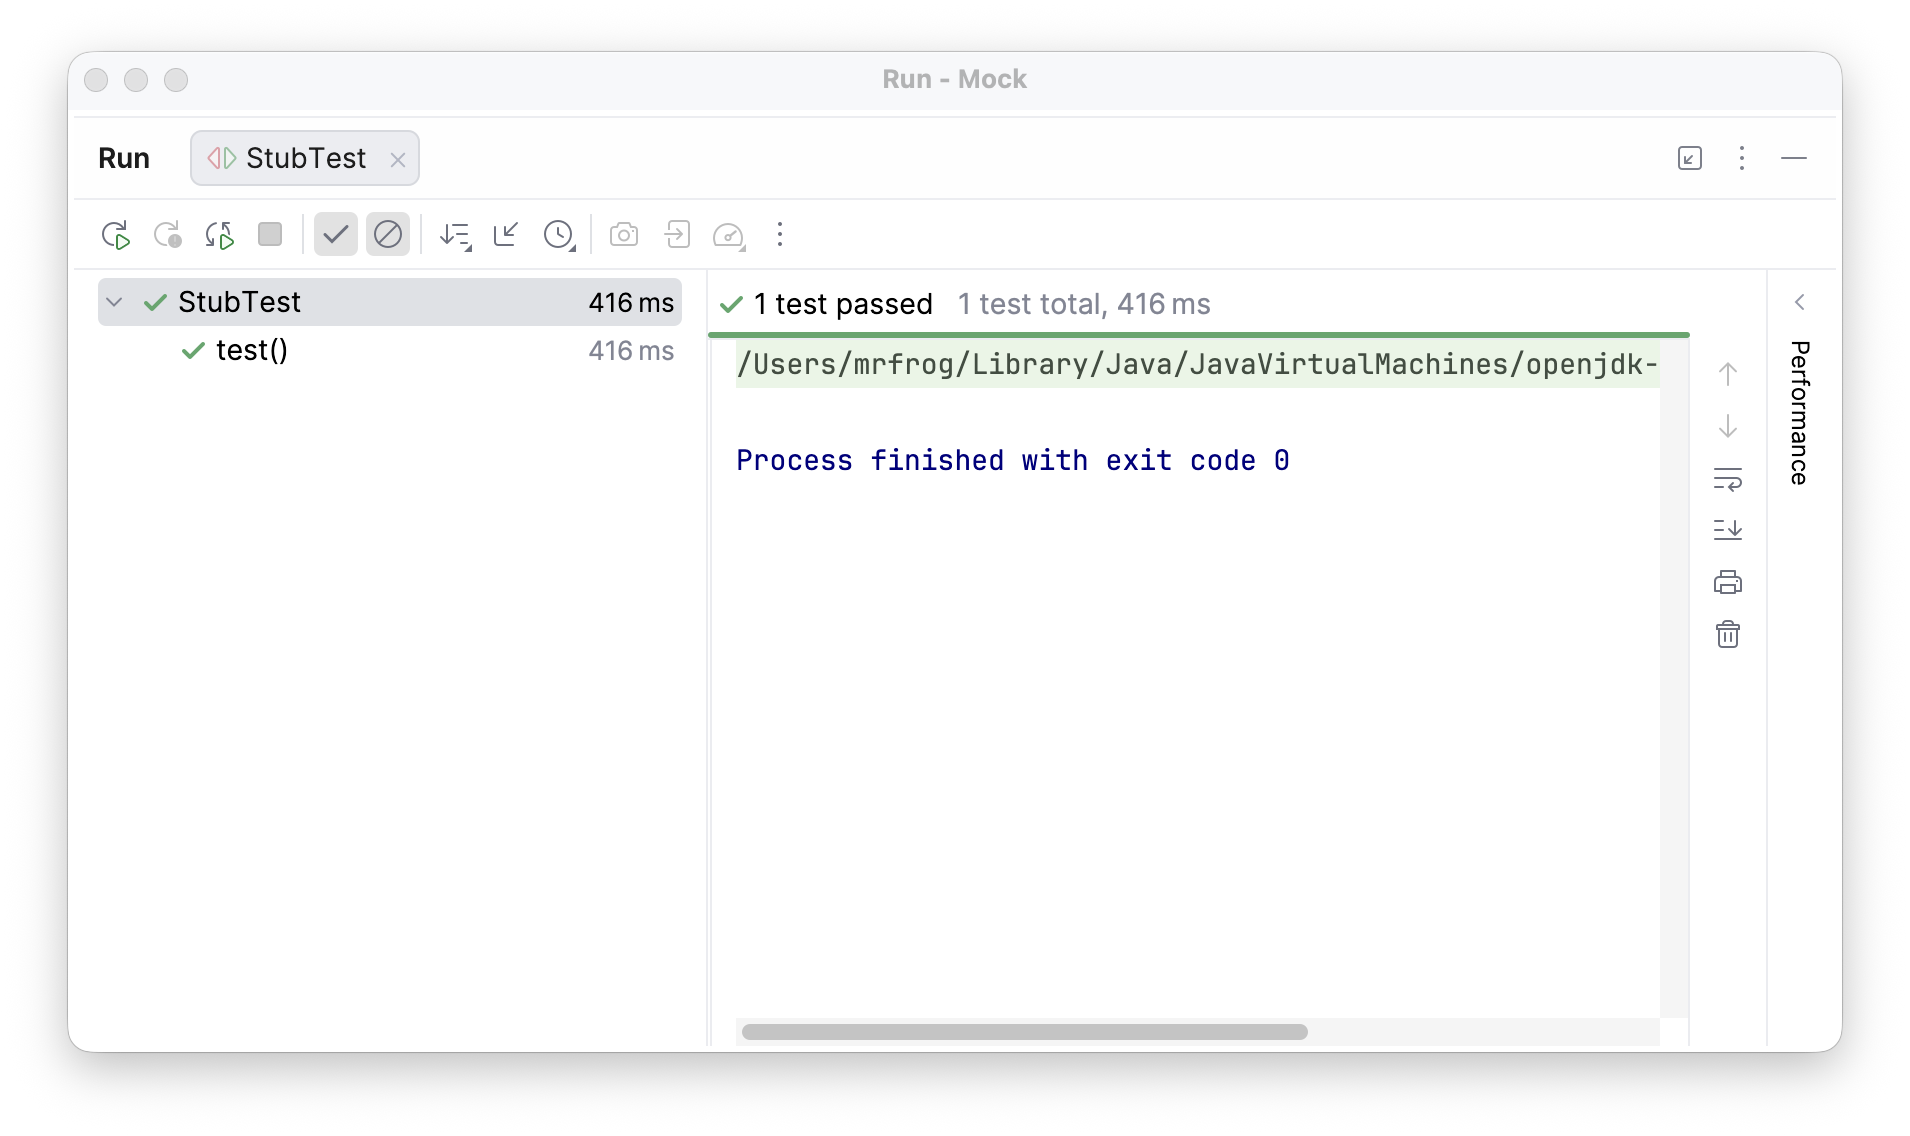
\includegraphics[width=0.9\textwidth]{stubtest.png}
    \caption{Hasil eksekusi StubTest}
\end{figure}

\clearpage

%----------------------------------------------------------------------
\section{Tugas}
%----------------------------------------------------------------------

Pada bagian tugas, dibuat skenario pengujian untuk sistem perpustakaan sederhana yang terdiri dari kelas \texttt{Book}, antarmuka \texttt{BookRepository} dan \texttt{NotificationService}, serta kelas \texttt{BookController}. Pengujian dilakukan menggunakan anotasi Mockito (\texttt{@Mock}, \texttt{@InjectMocks}, \texttt{@ExtendWith}).

% ---- Book Classes ----
\subsection{Kelas-Kelas Book}

Kelas \texttt{Book} merepresentasikan buku dengan atribut \texttt{id}, \texttt{title}, dan \texttt{available}.

\begin{lstlisting}[style=javastyle, caption={Book.java}]
package org.example;

public class Book {
    private String id;
    private String title;
    private boolean available;

    public Book(String id, String title, boolean available) {
        this.id = id;
        this.title = title;
        this.available = available;
    }

    public String getId()       { return id; }
    public String getTitle()    { return title; }
    public boolean isAvailable(){ return available; }
}
\end{lstlisting}

\texttt{BookRepository} adalah antarmuka yang mendefinisikan operasi \texttt{findById}, \texttt{findAll}, dan \texttt{peminjaman}.

\begin{lstlisting}[style=javastyle, caption={BookRepository.java}]
package org.example;

import java.util.List;
import java.util.Optional;

public interface BookRepository {
    Optional<Book> findById(String id);
    List<Book> findAll();
    void peminjaman(String title, String username);
}
\end{lstlisting}

\texttt{NotificationService} adalah antarmuka untuk mengirim notifikasi kepada pengguna.

\begin{lstlisting}[style=javastyle, caption={NotificationService.java}]
package org.example;

public interface NotificationService {
    void sendNotification(String username, String title);
}
\end{lstlisting}

\texttt{BookController} adalah kelas utama yang mengandung logika bisnis: pengecekan ketersediaan buku dan alur peminjaman.

\begin{lstlisting}[style=javastyle, caption={BookController.java}]
package org.example;

import java.util.List;

public class BookController {
    private final BookRepository repository;
    private final NotificationService notificationService;

    public BookController(BookRepository repository,
                          NotificationService notificationService) {
        this.repository = repository;
        this.notificationService = notificationService;
    }

    public boolean checkAvailability(String id) {
        return repository.findById(id)
                .map(Book::isAvailable)
                .orElse(false);
    }

    public void borrowBook(String id, String username) {
        List<Book> books = repository.findAll(); // Urutan 1

        Book book = repository.findById(id)
                .orElseThrow(() -> new RuntimeException("Book not found"));

        if (book.isAvailable()) {
            repository.peminjaman(book.getTitle(), username); // Urutan 2
            notificationService.sendNotification(username,
                                                 book.getTitle()); // Urutan 3
        }
    }
}
\end{lstlisting}

% ---- BookTest ----
\subsection{BookTest}

Kelas \texttt{BookTest} berisi tiga skenario pengujian yang menggabungkan teknik \textbf{Stub} (untuk men-\textit{stub} nilai kembalian) dan \textbf{Mock} (untuk verifikasi interaksi dan urutan pemanggilan). Berikut adalah struktur awal kelas beserta deklarasi dependensi yang di-\textit{inject} menggunakan anotasi Mockito.

\begin{lstlisting}[style=javastyle, caption={BookTest.java -- Deklarasi Kelas dan Anotasi}]
@ExtendWith(MockitoExtension.class)
public class BookTest {

    @Mock
    private BookRepository bookRepository;

    @Mock
    private NotificationService notificationService;

    @InjectMocks
    private BookController bookController;
}
\end{lstlisting}

Penjelasan deklarasi:
\begin{itemize}
    \item \texttt{@ExtendWith(MockitoExtension.class)} --- mengaktifkan ekstensi Mockito pada JUnit 5 sehingga anotasi \texttt{@Mock} dan \texttt{@InjectMocks} diproses otomatis sebelum setiap test.
    \item \texttt{@Mock} --- membuat objek mock untuk \texttt{BookRepository} dan \texttt{NotificationService} tanpa implementasi nyata.
    \item \texttt{@InjectMocks} --- membuat instansi \texttt{BookController} dan menyuntikkan mock di atas ke dalamnya secara otomatis.
\end{itemize}

% ---- Test 1 ----
\subsubsection{Test 1: testCheckAvailability\_Success}

Test ini memverifikasi bahwa \texttt{checkAvailability} mengembalikan \texttt{true} ketika buku dengan ID yang diminta tersedia.

\begin{lstlisting}[style=javastyle, caption={BookTest.java -- testCheckAvailability\_Success}]
@Test
void testCheckAvailability_Success() {
    Book book = new Book("B01", "Clean Code", true);
    when(bookRepository.findById("B01")).thenReturn(Optional.of(book));

    boolean available = bookController.checkAvailability("B01");

    assertTrue(available);
    verify(bookRepository).findById("B01");
}
\end{lstlisting}

Langkah-langkah pengujian:
\begin{enumerate}
    \item \textbf{Stub} --- \texttt{findById("B01")} dikonfigurasi agar mengembalikan \texttt{Optional} berisi buku dengan \texttt{available = true}.
    \item \textbf{Eksekusi} --- \texttt{checkAvailability("B01")} dipanggil pada \texttt{bookController}.
    \item \textbf{Verifikasi State} --- \texttt{assertTrue(available)} memastikan nilai kembalian adalah \texttt{true}.
    \item \textbf{Verifikasi Interaksi} --- \texttt{verify(bookRepository).findById("B01")} memastikan metode \texttt{findById} dipanggil tepat satu kali.
\end{enumerate}

% ---- Test 2 ----
\subsubsection{Test 2: testBorrowBook\_WhenAvailable\_ShouldCallPeminjamanAndNotify}

Test ini memverifikasi bahwa ketika buku tersedia, alur peminjaman berjalan dengan urutan yang benar: \texttt{findAll} → \texttt{peminjaman} → \texttt{sendNotification}.

\begin{lstlisting}[style=javastyle, caption={BookTest.java -- testBorrowBook\_WhenAvailable}]
@Test
void testBorrowBook_WhenAvailable_ShouldCallPeminjamanAndNotify() {
    String id = "B01";
    String username = "bangjan";
    Book book = new Book(id, "Clean Code", true);

    when(bookRepository.findAll())
            .thenReturn(Collections.singletonList(book));
    when(bookRepository.findById(id))
            .thenReturn(Optional.of(book));

    bookController.borrowBook(id, username);

    InOrder inOrder = inOrder(bookRepository, notificationService);
    inOrder.verify(bookRepository).findAll();
    inOrder.verify(bookRepository)
           .peminjaman("Clean Code", username);
    inOrder.verify(notificationService)
           .sendNotification(username, "Clean Code");
}
\end{lstlisting}

Langkah-langkah pengujian:
\begin{enumerate}
    \item \textbf{Stub} --- \texttt{findAll()} di-\textit{stub} mengembalikan list berisi satu buku, dan \texttt{findById(id)} mengembalikan buku yang sama dengan \texttt{available = true}.
    \item \textbf{Eksekusi} --- \texttt{borrowBook(id, username)} dipanggil, memicu seluruh alur peminjaman di dalam \texttt{BookController}.
    \item \textbf{Verifikasi Urutan (InOrder)} --- menggunakan \texttt{InOrder} untuk memastikan urutan pemanggilan tepat: pertama \texttt{findAll()}, kemudian \texttt{peminjaman("Clean Code", username)}, terakhir \texttt{sendNotification(username, "Clean Code")}.
\end{enumerate}

% ---- Test 3 ----
\subsubsection{Test 3: testBorrowBook\_WhenNotAvailable\_ShouldNotCallPeminjaman}

Test ini memverifikasi bahwa ketika buku tidak tersedia (\texttt{available = false}), metode \texttt{peminjaman} dan \texttt{sendNotification} tidak dipanggil sama sekali.

\begin{lstlisting}[style=javastyle, caption={BookTest.java -- testBorrowBook\_WhenNotAvailable}]
@Test
void testBorrowBook_WhenNotAvailable_ShouldNotCallPeminjaman() {
    String id = "B02";
    String username = "bangjan";
    Book book = new Book(id, "Design Patterns", false);

    when(bookRepository.findAll())
            .thenReturn(Collections.singletonList(book));
    when(bookRepository.findById(id))
            .thenReturn(Optional.of(book));

    bookController.borrowBook(id, username);

    verify(bookRepository).findAll();
    verify(bookRepository, never())
            .peminjaman(anyString(), anyString());
    verify(notificationService, never())
            .sendNotification(anyString(), anyString());
}
\end{lstlisting}

Langkah-langkah pengujian:
\begin{enumerate}
    \item \textbf{Stub} --- \texttt{findAll()} dan \texttt{findById(id)} di-\textit{stub} dengan buku yang memiliki \texttt{available = false}.
    \item \textbf{Eksekusi} --- \texttt{borrowBook(id, username)} dipanggil. Karena buku tidak tersedia, blok \texttt{if (book.isAvailable())} tidak dieksekusi.
    \item \textbf{Verifikasi Interaksi Negatif} --- \texttt{verify(..., never())} memastikan bahwa \texttt{peminjaman} dan \texttt{sendNotification} \textit{tidak pernah} dipanggil, mengonfirmasi bahwa logika kondisional berfungsi dengan benar.
\end{enumerate}

\begin{figure}[H]
    \centering
    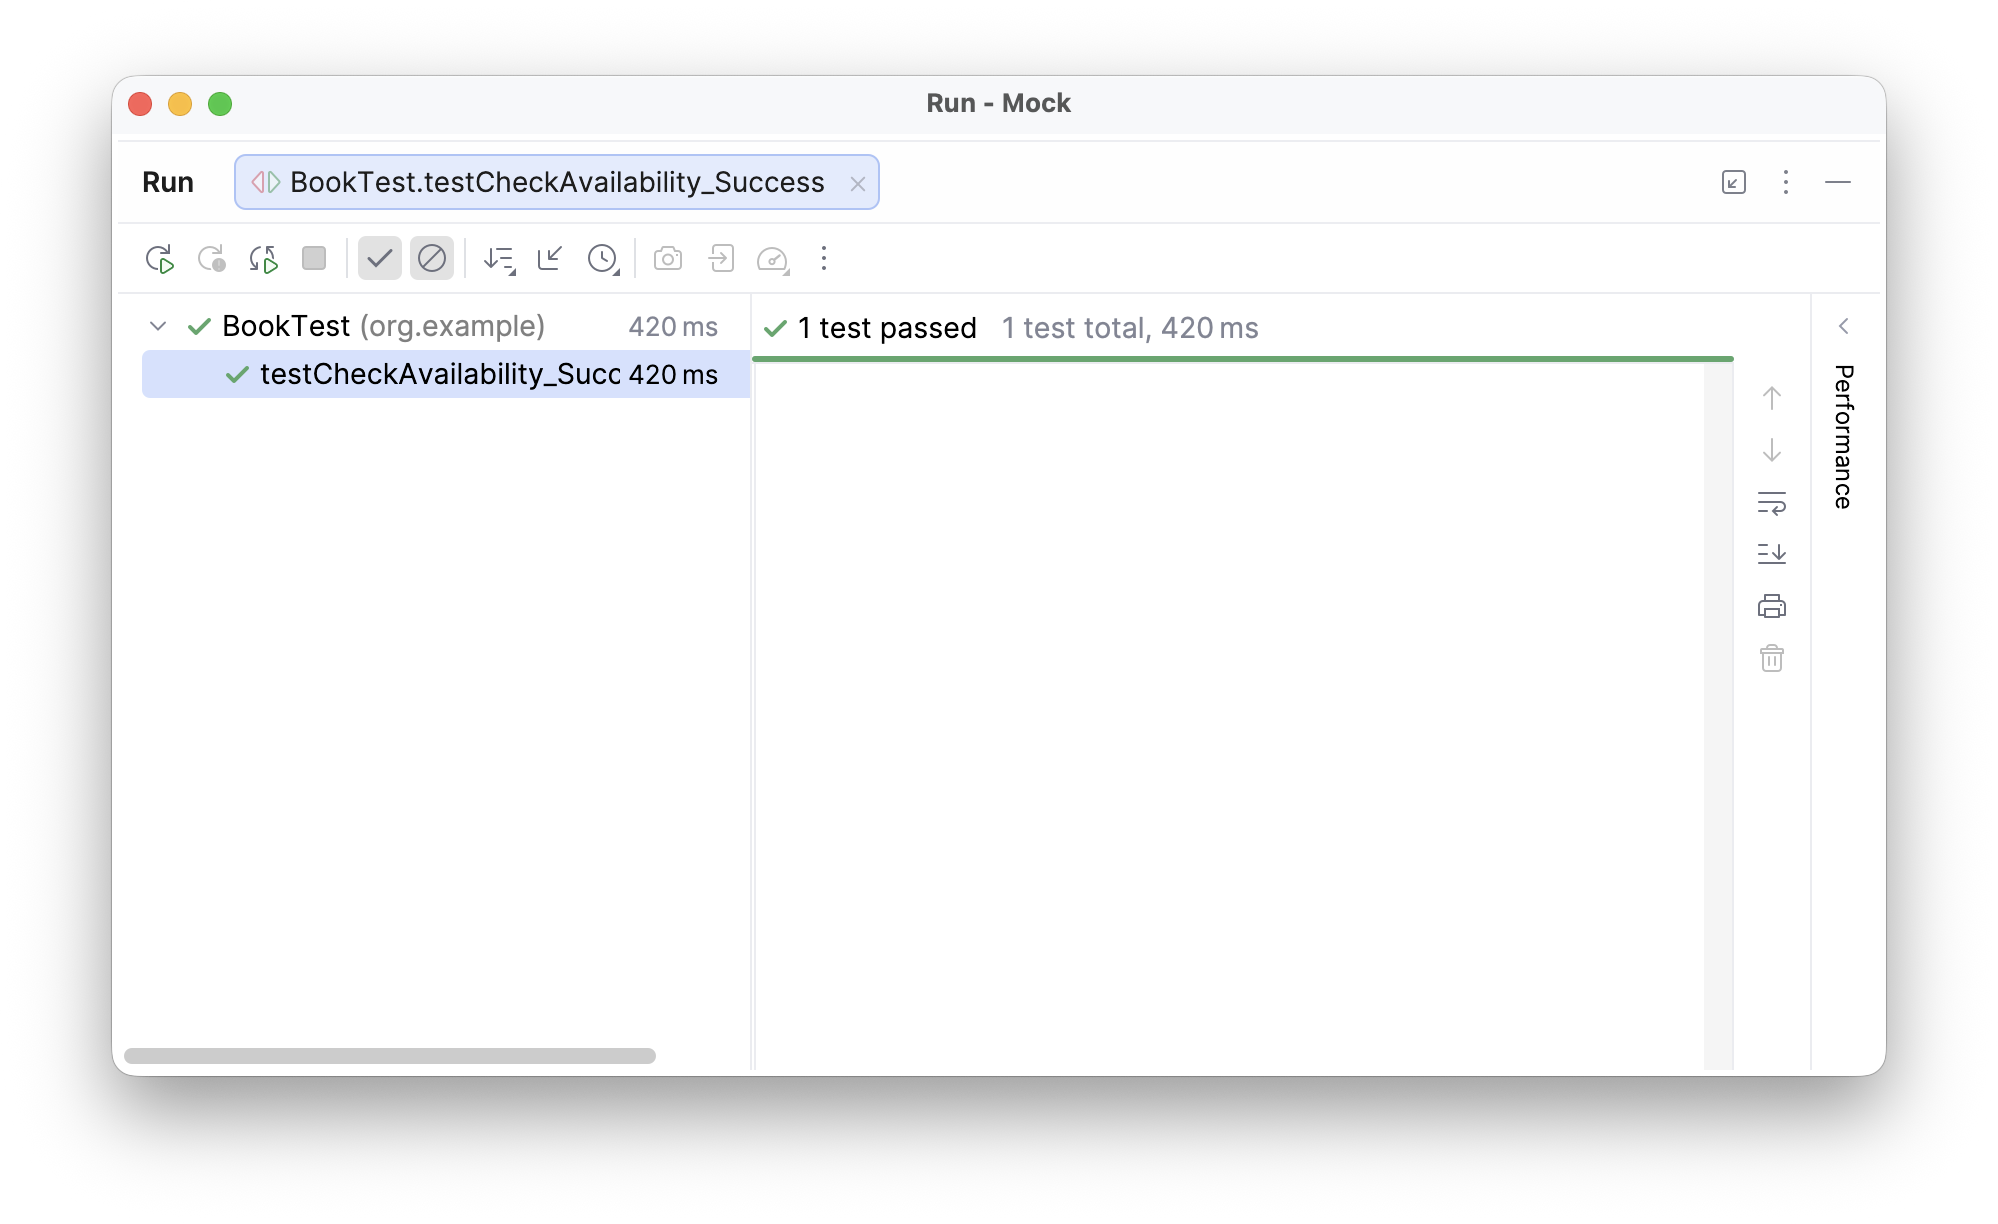
\includegraphics[width=0.9\textwidth]{booktest.png}
    \caption{Hasil eksekusi BookTest}
\end{figure}

\clearpage

%======================================================================
\chapter{Resources}
%======================================================================

\begin{center}
    \url{https://github.com/januarsyah901/PPPL/tree/9d622d374dcf5c9e04c560607ba4e59049f3681a/Pertemuan%204}
\end{center}

\clearpage

%======================================================================
\chapter{Kesimpulan}
%======================================================================

Berdasarkan praktikum yang telah dilakukan, dapat disimpulkan beberapa hal berikut:

Berdasarkan praktikum yang telah dilakukan, pengujian dengan Mockito menunjukkan bahwa \textbf{Mock} efektif untuk memverifikasi \textit{interaksi} antara unit yang diuji dan dependensinya, misalnya untuk memastikan suatu metode dipanggil atau tidak dipanggil dengan argumen tertentu. Sementara itu, \textbf{Spy} membungkus objek nyata sehingga implementasi asli tetap berjalan, sehingga pendekatan ini sesuai ketika pengujian membutuhkan verifikasi interaksi sekaligus perilaku asli objek. Di sisi lain, \textbf{Stub} berperan untuk mengatur nilai kembalian metode tertentu agar pengujian berfokus pada \textit{verifikasi state} hasil eksekusi, bukan pada mekanisme pemanggilan dependensi. Secara keseluruhan, kombinasi Mock dan Stub seperti pada \texttt{BookTest} menghasilkan pengujian yang lebih komprehensif karena mampu mencakup verifikasi nilai, verifikasi interaksi, serta verifikasi urutan pemanggilan metode menggunakan \texttt{InOrder}.

\clearpage
\addcontentsline{toc}{chapter}{Daftar Pustaka}
\renewcommand{\bibname}{Daftar Pustaka}

\begin{thebibliography}{99}
    \bibitem{mockito} Mockito Project, ``Mockito --- tasty mocking framework for unit tests in Java''. [Online]. Tersedia: \url{https://site.mockito.org/}.
    \bibitem{junit5} JUnit Team, ``JUnit 5 User Guide''. [Online]. Tersedia: \url{https://junit.org/junit5/docs/current/user-guide/}.
    \bibitem{fowler-mocks} Martin Fowler, ``Mocks Aren't Stubs'', 2007. [Online]. Tersedia: \url{https://martinfowler.com/articles/mocksArentStubs.html}.
\end{thebibliography}

\end{document}
